\documentclass[masc,grad]{coppe} %Universal input encoding G.L.
% \documentclass[aprovado,masc,grad]{coppe} %Universal input encoding G.L.
\maxdeadcycles=20
\usepackage[utf8]{inputenc}
\usepackage[english]{babel}
% \usepackage[brazil]{babel}
\usepackage[T1]{fontenc}
\usepackage{graphicx}
\usepackage{pax}
\usepackage{tikzscale}
\usepackage{appendix}
\usepackage{pgfplots}
\pgfplotsset{compat=newest}
\usepgfplotslibrary{groupplots}
\usepgfplotslibrary{dateplot}
\usepackage{xargs}
\usepackage{rotating}
\usepackage{pdflscape}
\usepackage{afterpage}
\usepackage[paper=A4,pagesize]{typearea}
\graphicspath{{../../figures/}} 
\usepackage{subcaption} 
\usepackage{hyperref}
\usepackage{amsmath,amssymb} 
\usepackage{indentfirst}
\usepackage[algo2e,linesnumbered,ruled]{algorithm2e}
\usepackage{algorithmic}
%%If desirable, the user can enable Times New Roman Fonts by uncommenting the next line. G.L.
% \usepackage{mathptmx}
\usepackage{pdfpages}
\usepackage{multirow}
\usepackage{color}
\usepackage{blindtext}
\usepackage{float}
\usepackage{nameref}
\usepackage{cleveref}
\usepackage{multicol}
\usepackage{listings}
\usepackage{enumerate}
\usepackage[acronym,toc]{glossaries}\makeglossaries
\usepackage{tikz}
\usepackage{ladder} %https://github.com/AurelienC/tex-ladder/blob/master/ladder.sty
\usetikzlibrary{arrows,shapes,automata,petri,external,arrows.meta}
	\tikzset{
	place/.style={
	circle,
	thick,
	draw=black!100, % draw=blue!75,
    % fill=blue!20,
    minimum size=6mm
  },
  extPlace/.style={
    circle,
    dotted,
    draw=black!100, % draw=blue!75,
    % fill=blue!20,
    minimum size=6mm
  },
  extTransition/.style={
    rectangle,
    dotted,
    fill=white,
    minimum width=8mm,
    inner ysep=0.7pt
  },
  transition/.style={
    rectangle,
    thick,
    fill=black,
    minimum width=8mm,
    inner ysep=0.7pt
  },
  extTimedtransition/.style={
    rectangle,
    dotted,
    fill=white,
    minimum width=8mm,
    inner ysep=2pt
  },
  timedtransition/.style={
    rectangle,
    thick,
    fill=white,
    minimum width=8mm,
    inner ysep=2pt
  },
  inhibitor/.style={-o},
  text/.style={}
}

\makeatletter
\tikz@def@grow@tokens{2}{1}{-1.5}{0}
\tikz@def@grow@tokens{2}{2}{1.5}{0}
% \tikz@def@grow@tokens{3}{1}{-1}{0}
% \tikz@def@grow@tokens{3}{2}{0}{1}
% \tikz@def@grow@tokens{3}{3}{1.5}{-1}
\makeatother


\definecolor{darkblue}{rgb}{0,0,0.3}
\definecolor{blue}{rgb}{0,0,0.5}
\definecolor{color1}{rgb}{1,0.2,0.3}
\definecolor{color2}{rgb}{0.05490196078,0.41176470588,0.13333333333}
% rgb(14, 105, 34)

\definecolor{color3}{rgb}{0.2,0.2,0.8}
% hyperref setup
\hypersetup{
  % pdftitle={\title},
  pdfauthor={Rafael Accácio Nogueira},
  pdfcreator={Rafael Accácio Nogueira},     
  bookmarksopen=true,         
  bookmarksopenlevel=1,       
  colorlinks=true, % false => boxes 
  linkcolor=blue,
  filecolor=red,  
  urlcolor=blue,  
  citecolor=blue,              
  pdfstartview=Fit,          
  pdfpagemode=UseOutlines,    % this is the option you were lookin for
  pdfpagelayout=TwoPageRight,
}

\makeatletter
\let\stdchapter\chapter
\renewcommand*\chapter{%
  \@ifstar{\starchapter}{\@dblarg\nostarchapter}}
\newcommand*\starchapter[1]{\stdchapter*{#1}}
\def\nostarchapter[#1]#2{
  \stdchapter[#1]{\protect\hyperlink{tocsection}{#1}}}
\makeatother

\makeatletter
\let\stdsection\section
\renewcommand*\section{%
  \@ifstar{\starsection}{\@dblarg\nostarsection}}
\newcommand*\starsection[1]{\stdsection*{#1}}
\def\nostarsection[#1]#2{
  \stdsection[#1]{\protect\hyperlink{tocsection}{#1}}}
\makeatother

\makeatletter
\let\stdsubsection\subsection
\renewcommand*\subsection{%
  \@ifstar{\starsubsection}{\@dblarg\nostarsubsection}}
\newcommand*\starsubsection[1]{\stdsubsection*{#1}}
\def\nostarsubsection[#1]#2{
  \stdsubsection[#1]{\protect\hyperlink{tocsection}{#1}}}
\makeatother

\makeatletter
\let\stdsubsubsection\subsubsection
\renewcommand*\subsubsection{%
  \@ifstar{\starsubsubsection}{\@dblarg\nostarsubsubsection}}
\newcommand*\starsubsubsection[1]{\stdsubsubsection*{#1}}
\def\nostarsubsubsection[#1]#2{
  \stdsubsubsection[#1]{\protect\hyperlink{tocsection}{#1}}}
\makeatother

\let\oldtoc\tableofcontents
\renewcommand{\tableofcontents}{\pagebreak\hypertarget{tocsection}{}\label{tocsection}\oldtoc}


\newcommand{\figplaceholder}[2]{
	\begin{figure}[H]
		\begin{center}	
			\rule{8cm}{8cm}
			\caption{\todo[FORGOT TO INCLUDE FIGURE]{#1 (placeholder)}}
			\label{fig:#2}
		\end{center}
	\end{figure}
}

\newif\ifdebug
\newcommand{\draft}{\debugtrue}
\newcommand{\final}{\debugfalse}
\newcommand{\todo}[2][FORGOT TO DO SOMETHING]{\ifdebug {\color{red}#2}\else \PackageError{}{#1}{}\fi}
\newcommand\doing[1]{\ifdebug {\color{blue}#1}\else \PackageError{}{FORGOT TO DO SOMETHING}{}\fi}
\newcommand\warning[1]{\ifdebug {\color{red}#1}\fi}
\newcommand\note[1]{\ifdebug {\color{orange}#1}\fi}

\usepackage{fancyhdr}
\pagestyle{fancy}

\fancyhead[L]{\warning{DRAFT}}
\fancyhead[R]{\warning{DEBUG ON}}

\fancyfoot[L]{\warning{TURN DEBUG OFF}}
\fancyfoot[R]{\warning{DRAFT}}

\newtheorem{theorem}{Theorem}
\numberwithin{theorem}{chapter}

\newtheorem{example}{Example}
\numberwithin{example}{chapter}

\newtheorem{definition}{Definition}
\numberwithin{definition}{chapter}

\newtheorem{observation}{Remark}
\numberwithin{observation}{chapter}

\usepackage[export]{adjustbox}

\newcommand{\includetikzfigure}[2][]{
    \ifdebug {\includegraphics[#1]{#2.pdf}}
    \else  \includegraphics[#1]{#2}\fi
}

\newcommand{\addtikzfigureLandscape}[4][width=0.8\textwidth]{
\KOMAoptions{paper=landscape}
\recalctypearea
  \vspace*{\fill}
  \begin{figure}[H]
    \centering
    \ifdebug {\includegraphics[#1]{#2.pdf}}
    \else  \includegraphics[#1]{#2}\fi
    \caption{#3}
    \label{fig:#4}
  \end{figure}
  \vspace*{\fill}
\KOMAoptions{paper=portrait}
\recalctypearea
}

\newcommand{\addtikzfigureLandscapeAthree}[4][width=0.8\textwidth]{
\KOMAoptions{paper=a3,paper=landscape}
% \KOMAoptions{paper=landscape}
\recalctypearea
  \begin{figure}[H]
    \vspace{-2cm}
    \centering
    \ifdebug {\centerline{\includegraphics[#1]{#2.pdf}}}
    \else  \centerline{\includegraphics[#1]{#2}}
\fi
    % \caption{#3}
    % \label{fig:#4}
  \end{figure}
\KOMAoptions{paper=a4,paper=portrait}
\recalctypearea
}

% \newcommand{\addtikzfigureVertCent}[3]{
% \KOMAoptions{paper=landscape}
% \recalctypearea
% % \begin{landscape}
% \vspace*{\fill}
%   \begin{figure}[H]
%     % \centering
%     % \resizebox{\hsize}{!}{
%     % \input{#1}
%      \includegraphics[width=1.15\textwidth]{#1}
%     % }
%     \caption{#2}
%     \label{fig:#3}
%   \end{figure}
% \vspace*{\fill}
% % \end{landscape}
% \KOMAoptions{paper=portrait}
% \recalctypearea
% }

\newcolumntype{P}[1]{>{\centering\arraybackslash}p{#1}}
\newcolumntype{M}[1]{>{\centering\arraybackslash}m{#1}}
\definecolor{keywordstyle}{rgb}{0,0,0.82}
\definecolor{commentstyle}{rgb}{0,0.6,0}
\definecolor{numberstyle}{rgb}{0.5,0.5,0.5}
\definecolor{stringstyle}{rgb}{0.58,0,0.82}

% Listing options
\lstset{ 
  % backgroundcolor=\color{white},   % choose the background color; you must add \usepackage{color} or \usepackage{xcolor}; should come as last argument
  basicstyle=\footnotesize,        % the size of the fonts that are used for the code
  breakatwhitespace=false,         % sets if automatic breaks should only happen at whitespace
  breaklines=true,                 % sets automatic line breaking
  captionpos=t,                    % sets the caption-position to bottom
  commentstyle=\color{commentstyle},    % comment style
  deletekeywords={...},            % if you want to delete keywords from the given language
  escapeinside={\%*}{*)},          % if you want to add LaTeX within your code
  extendedchars=true,              % lets you use non-ASCII characters; for 8-bits encodings only, does not work with UTF-8
  % firstnumber=1000,                % start line enumeration with line 1000
  % frame=single,	                   % adds a frame around the code
  keepspaces=true,                 % keeps spaces in text, useful for keeping indentation of code (possibly needs columns=flexible)
  keywordstyle=\color{keywordstyle},       % keyword style
  % language=Octave,                 % the language of the code
  morekeywords={*,...},            % if you want to add more keywords to the set
  numbers=left,                    % where to put the line-numbers; possible values are (none, left, right)
  numbersep=10pt,                   % how far the line-numbers are from the code
  numberstyle=\tiny\color{numberstyle}, % the style that is used for the line-numbers
  rulecolor=\color{black},         % if not set, the frame-color may be changed on line-breaks within not-black text (e.g. comments (green here))
  showspaces=false,                % show spaces everywhere adding particular underscores; it overrides 'showstringspaces'
  showstringspaces=false,          % underline spaces within strings only
  showtabs=false,                  % show tabs within strings adding particular underscores
  stepnumber=2,                    % the step between two line-numbers. If it's 1, each line will be numbered
  stringstyle=\color{stringstyle},     % string literal style
  tabsize=2,	                   % sets default tabsize to 2 spaces
  title=\lstname                   % show the filename of files included with \lstinputlisting; also try caption instead of title
}

%% as seen in https://tex.stackexchange.com/a/183682/143332
\makeatletter
\newcommand\Autoref[1]{\@first@ref#1,@}
\def\@throw@dot#1.#2@{#1}% discard everything after the dot
\def\@set@refname#1{%    % set \@refname to autoefname+s using \getrefbykeydefault
    \edef\@tmp{\getrefbykeydefault{#1}{anchor}{}}%
    \xdef\@tmp{\expandafter\@throw@dot\@tmp.@}%
    \ltx@IfUndefined{\@tmp autorefnameplural}%
         {\def\@refname{\@nameuse{\@tmp autorefname}s}}%
         {\def\@refname{\@nameuse{\@tmp autorefnameplural}}}%
}
\def\@first@ref#1,#2{%
  \ifx#2@\autoref{#1}\let\@nextref\@gobble% only one ref, revert to normal \autoref
  \else%
    \@set@refname{#1}%  set \@refname to autoref name
    \@refname~\ref{#1}% add autoefname and first reference
    \let\@nextref\@next@ref% push processing to \@next@ref
  \fi%
  \@nextref#2%
}
\def\@next@ref#1,#2{%
   \ifx#2@ and~\ref{#1}\let\@nextref\@gobble% at end: print and+\ref and stop
   \else, \ref{#1}% print  ,+\ref and continue
   \fi%
   \@nextref#2%
 }
 \makeatother

\newcommand{\colvec}[2][1]{%
  \scalebox{#1}{%
    \renewcommand{\arraystretch}{.7}%
    $\begin{bmatrix}#2\end{bmatrix}$%
  }
}


%%% Local Variables:
%%% mode: latex
%%% TeX-master: "./monografia.tex"
%%% End:


\newcommandx\acr[5][4=,5=]{
  \ifthenelse{\equal{#5}{}}
  {
    \acrSing{#1}{#2}{#3}
  }
  {
    \acrPl{#1}{#2}{#3}{#4}{#5}
  }
  } 

\newcommand{\acrSing}[3]{\newacronym{#1}{#2}{#3}
  \expandafter\newcommand\csname #1\endcsname{\gls{#1}}}

\newcommand{\acrPl}[5]{
  \newacronym[plural=#4,firstplural=#5 (#4)]{#1}{#2}{#3}
  \expandafter\newcommand\csname #1\endcsname{\gls{#1}}
  \expandafter\newcommand\csname #4\endcsname{\glspl{#1}}
}

\renewcommand{\symbl}[3]{\newglossaryentry{#1}{name ={#2},	description ={#3}}
  \expandafter\newcommand\csname #1\endcsname{\gls{#1}}
}


\newglossarystyle{dottedlocations}{%
   \glossarystyle{list}%
   \renewcommand*{\glossaryentryfield}[5]{%
   \item[\glsentryitem{##1}\glstarget{##1}{##2}] ##3, p %
       \unskip\leaders\hbox to 2.9mm{} ##5}%
   \renewcommand*{\glsgroupskip}{}%
}

 \newglossarystyle{acronyms}{%
 % put the glossary in the itemize environment:
 \renewenvironment{theglossary}%
   {\begin{tabbing}}{\end{tabbing}}%
 % have nothing after \begin{theglossary}:
 \renewcommand*{\glossaryheader}{}%
 % have nothing between glossary groups:
 \renewcommand*{\glsgroupheading}[1]{}%
 \renewcommand*{\glsgroupskip}{}%
 % set how each entry should appear:
 \renewcommand*{\glossentry}[2]{%
 \glstarget{##1}{\glossentryname{##1}}\\% \kill % the entry name
 \=\glossentrysymbol{##1}% the symbol in brackets
 \space \glossentrydesc{##1},% the description
 \space p. ##2\\% the number list in square brackets
 }%
 % set how sub-entries appear:
 \renewcommand*{\subglossentry}[3]{%
   \glossentry{##2}{##3}}%
}


 \newglossarystyle{symbols}{%
 % put the glossary in the itemize environment:
 \renewenvironment{theglossary}%
   {\begin{tabbing}}{\end{tabbing}}%
 % have nothing after \begin{theglossary}:
 \renewcommand*{\glossaryheader}{}%
 % have nothing between glossary groups:
 \renewcommand*{\glsgroupheading}[1]{}%
 \renewcommand*{\glsgroupskip}{}%
 % set how each entry should appear:
 \renewcommand*{\glossentry}[2]{%
 \glstarget{##1}{\glossentryname{##1}}\\% \kill % the entry name
 \=\textbf{\glossentrysymbol{##1}}% the symbol in brackets
 
 \space \glossentrydesc{##1},% the description
 \space p. ##2\\% the number list in square brackets
 }%
 % set how sub-entries appear:
 \renewcommand*{\subglossentry}[3]{%
   \glossentry{##2}{##3}}%
 }


\acr{DAOCT}{DAOCT}{Deterministic Automaton
  with Outputs and Conditional Transitions}
\acr{ECA}{ECA}{Engenharia de controle e Automação}
\acr{PLC}{PLC}{Programmable Logic Controller}
[PLCs][Programmable Logic Controllers]
\acr{DES}{DES}{Discrete Event System}
[DESs][Discrete Event Systems]


\acr{LD}{LD}{Ladder Diagram}

\acr{CIPN}{CIPN}{Control Interpreted Petri Net}

% DAOCT
\symbl{OmegaSet}{$\Omega$}{$\Omega \subset \mathbb{N}_1^{m_i + m_0}$ Set of IO vectors}
\symbl{SigmaSet}{$\Sigma$}{Set of events}
\symbl{XSet}{$X$}{Set of states}
\symbl{ffunction}{$f$}{$f : X \times \Sigma^* \rightarrow X$ Deterministic
  transition function}
\symbl{lambdafunction}{$\lambda$}{$\lambda : X \rightarrow \Omega$ State
  output function}
\symbl{RSet}{$R$}{$R = \{1,2,\dots,r\} $ Set of path indices}
\symbl{thetafunction}{$\theta$}{$\theta : X \times \Sigma \rightarrow 2^R$ Path
  estimation function}
\symbl{xZero}{$x_0$}{Initial State}
\symbl{XfSet}{$X_f$}{$X_f \subseteq X$ Set of final states}
%%% Local Variables:
%%% mode: latex
%%% TeX-master: "./monografia.tex"
%%% End:
\makeindex
\makelosymbols
\makeloabbreviations
\acr{ECA}{ECA}{Engenharia de controle e Automação}
% \final
\draft

% include only to speed up tests
% \includeonly{test/examples}
\signedFrontPage{../../figures/poli-logo.pdf}

\begin{document}
% Identificação e Detecção de Falhas em um Sistema de Manufatura Didático
\title{Identification and Failure~Detection in a Didactic~Manufacture~System}
\foreigntitle{Identificação e Detecção~de~Falhas em um Sistema~de~Manufatura~Didático}
\author{Rafael Accácio}{Nogueira}

\advisor{Prof.}{Marcos Vicente de Brito}{Moreira}{D.Sc.}


% Case advisor is a woman add {f} Example:
% \advisor{Prof.}{Marie}{Sklodowksca-Curie}{PhD.}{f}

% \advisor{Prof.}{Nome do Segundo Orientador}{Sobrenome}{Ph.D.}
% \advisor{Prof.}{Nome do Terceiro Orientador}{Sobrenome}{D.Sc.}

% \examiner{Prof.}{Nome do Primeiro Examinador Sobrenome}{D.Sc.}
% \examiner{Prof.}{Nome do Segundo Examinador Sobrenome}{Ph.D.}
% \examiner{Prof.}{Nome do Terceiro Examinador Sobrenome}{D.Sc.}
\department{ECA}

\date{04}{2019}

\keyword{Failure~Detection}
\keyword{Discrete~Event~Systems}
\maketitle

\frontmatter


\makefrontpage\warning{TURN DEBUG OFF}\newpage


\makecatalog
\dedication{“It's a dangerous business going out your door. You step onto the road,
and if you don't keep your feet, there's no knowing where you might be swept off
to.” \\(J.R.R Tolkien)}
% ``É um negócio perigoso, Frodo, sair da sua porta. Você pisa na estrada, e, se
% não controlar seus pés, não há como saber até onde você pode ser levado''
% ``Se enxerguei mais longe, foi porque me apoiei sobre os ombros de gigantes.'' (Isaac Newton)

%%% Local Variables:
%%% mode: latex
%%% TeX-master: "../monografia.tex"
%%% End:

\include{frontMatter/thanks}

\begin{abstract}

Apresenta-se, nesta tese, ...

\end{abstract}
\begin{foreignabstract}

In this work, we present ...

\end{foreignabstract}

\tableofcontents

\listoffigures
\listoftables
\printlosymbols
\printloabbreviations
\setglossarystyle{long4col}
\renewcommand*{\glsnamefont}[1]{\textmd{#1}}

\newglossarystyle{dottedlocations}{%
   \glossarystyle{list}%
   \renewcommand*{\glossaryentryfield}[5]{%
   \item[\glsentryitem{##1}\glstarget{##1}{##2}] ##3, p %
       \unskip\leaders\hbox to 2.9mm{} ##5}%
   \renewcommand*{\glsgroupskip}{}%
}

 \newglossarystyle{tabular}{%
 % put the glossary in the itemize environment:
 \renewenvironment{theglossary}%
   {\begin{tabular}{ll}}{\end{tabular}}%
 % have nothing after \begin{theglossary}:
 \renewcommand*{\glossaryheader}{}%
 % have nothing between glossary groups:
 \renewcommand*{\glsgroupheading}[1]{}%
 \renewcommand*{\glsgroupskip}{}%
 % set how each entry should appear:
 \renewcommand*{\glossentry}[2]{%

 \glstarget{##1}{\glossentryname{##1}}&% the entry name
  \glossentrysymbol{##1}% the symbol in brackets
 \space \glossentrydesc{##1},% the description
 \space p. ##2\\% the number list in square brackets
 }%
 % set how sub-entries appear:
 \renewcommand*{\subglossentry}[3]{%
   \glossentry{##2}{##3}}%
}

 \newglossarystyle{mylist}{%
 % put the glossary in the itemize environment:
 \renewenvironment{theglossary}%
   {\begin{tabbing}}{\end{tabbing}}%
 % have nothing after \begin{theglossary}:
 \renewcommand*{\glossaryheader}{}%
 % have nothing between glossary groups:
 \renewcommand*{\glsgroupheading}[1]{}%
 \renewcommand*{\glsgroupskip}{}%
 % set how each entry should appear:
 \renewcommand*{\glossentry}[2]{%

 \glstarget{##1}{\glossentryname{##1}}\\% \kill % the entry name
 \=\glossentrysymbol{##1}% the symbol in brackets
 \space \glossentrydesc{##1},% the description
 \space p. ##2\\% the number list in square brackets
 }%
 % set how sub-entries appear:
 \renewcommand*{\subglossentry}[3]{%
   \glossentry{##2}{##3}}%
 }

\glossarystyle{mylist}

\newacronym{manet}{MANET}{Mobile Ad hoc NETwork}
\newacronym{rwp}{RWP}{Random WayPoint}
\newacronym{rw}{RW}{Random Walk}
\glsaddall

\printglossary[type=\acronymtype]\newpage
\printglossary[]

\newpage

\mainmatter


\chapter{Examples}
\label{chap:examples}

\section{teste}
\subsection{teste}
\subsubsection{teste}
\begin{figure}[H]
  \centering
  \begin{tikzpicture}
    \node[anchor=south west,inner sep=0] (image) at (0,0) {
      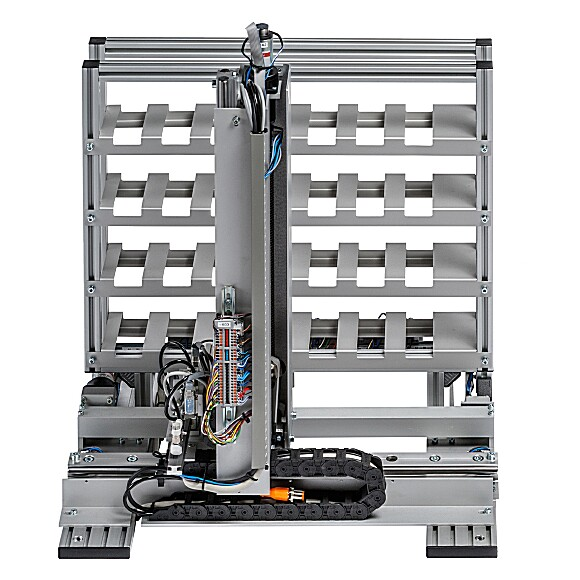
\includegraphics[width=8cm]{maquete/elevador/69523_3.jpg}
    };
    % \draw[red,ultra thick,rounded corners] (0,0) rectangle (9.4,6.2);
    \begin{scope}[x={(image.south east)},y={(image.north west)}]
        % \draw[help lines,xstep=.1,ystep=.1] (0,0) grid (1,1);
        % \foreach \x in {0,1,...,9} { \node [anchor=north] at (\x/10,0) {0.\x}; }
        % \foreach \y in {0,1,...,9} { \node [anchor=east] at (0,\y/10) {0.\y}; }
      \draw[red] (1,0.5) node {\textbf{Right}};
      \draw[red] (0,0.5) node {\textbf{Left}};
      \draw[red] (0.5,1) node {\textbf{Top}};
      \draw[red] (0.5,0) node {\textbf{Bottom}};
      \end{scope}
  \end{tikzpicture}
  \caption{Storage Unit}
\end{figure}


\begin{figure}[H]
  \centering
  \begin{tikzpicture}
    \node[anchor=south west,inner sep=0] (image) at (0,0) {
      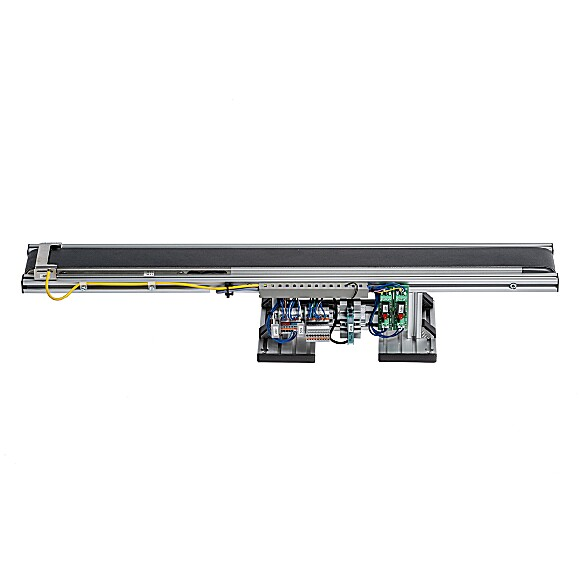
\includegraphics[trim={0 6cm 0 5cm},clip,width=8cm]{maquete/esteira/40778_3.jpg}
    };
    % \draw[red,ultra thick,rounded corners] (0,0) rectangle (9.4,6.2);
    \begin{scope}[x={(image.south east)},y={(image.north west)}]
        % \draw[help lines,xstep=.1,ystep=.1] (0,0) grid (1,1);
        % \foreach \x in {0,1,...,9} { \node [anchor=north] at (\x/10,0) {0.\x}; }
        % \foreach \y in {0,1,...,9} { \node [anchor=east] at (0,\y/10) {0.\y}; }
        \draw [->,>=stealth,red, very thick](0.9,0.7) -- (0.1,0.7);
        \draw [red] (0.5,0.8) node {Forward};
        \draw [->,>=stealth,red, very thick](0.1,0.1) -- (0.9,0.1);
        \draw [red](0.5,0.0) node {Reverse};
      \end{scope}
  \end{tikzpicture}
  \caption{Conveyor Belt}
\end{figure}

\begin{figure}[H]
  \centering
  \begin{tikzpicture}
    \node[anchor=south west,inner sep=0] (image) at (0,0) {
      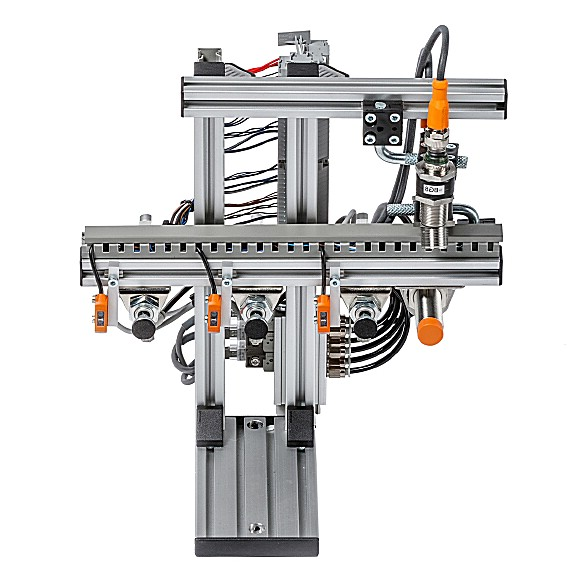
\includegraphics[trim={0 0 0 0},clip,width=8cm]{maquete/sensores/69511_3.jpg}
    };
    % \draw[red,ultra thick,rounded corners] (0,0) rectangle (9.4,6.2);
    \begin{scope}[x={(image.south east)},y={(image.north west)}]
        % \draw[help lines,xstep=.1,ystep=.1] (0,0) grid (1,1);
        % \foreach \x in {0,1,...,9} { \node [anchor=north] at (\x/10,0) {0.\x}; }
        % \foreach \y in {0,1,...,9} { \node [anchor=east] at (0,\y/10) {0.\y};  }
        \draw[red,ultra thick,rounded corners] (0.15,0.4) rectangle ++ (0.15,0.1);
        \draw[red] (0.1,0.1) node {\textbf{Left}};
        \draw[->,>=stealth,red, very thick] (0.2,0.38) -- (0.1,0.15);
        \draw[magenta,ultra thick,rounded corners] (0.35,0.4) rectangle ++ (0.15,0.1);
        \draw[magenta] (0.1,0.8) node {\textbf{Center}};
        \draw[->,>=stealth,magenta, very thick] (0.4,0.52) -- (0.2,0.75);
        \draw[cyan,ultra thick,rounded corners] (0.53,0.4) rectangle ++ (0.15,0.1);
        \draw[cyan] (0.7,0.1) node {\textbf{Right}};
        \draw[->,>=stealth,cyan, very thick] (0.65,0.38) -- (0.7,0.15);
      \end{scope}
  \end{tikzpicture}
  \caption{Sensors}
\end{figure}

\begin{figure}[H]
  \centering
  \begin{tikzpicture}
    \node[anchor=south west,inner sep=0] (image) at (0,0) {
      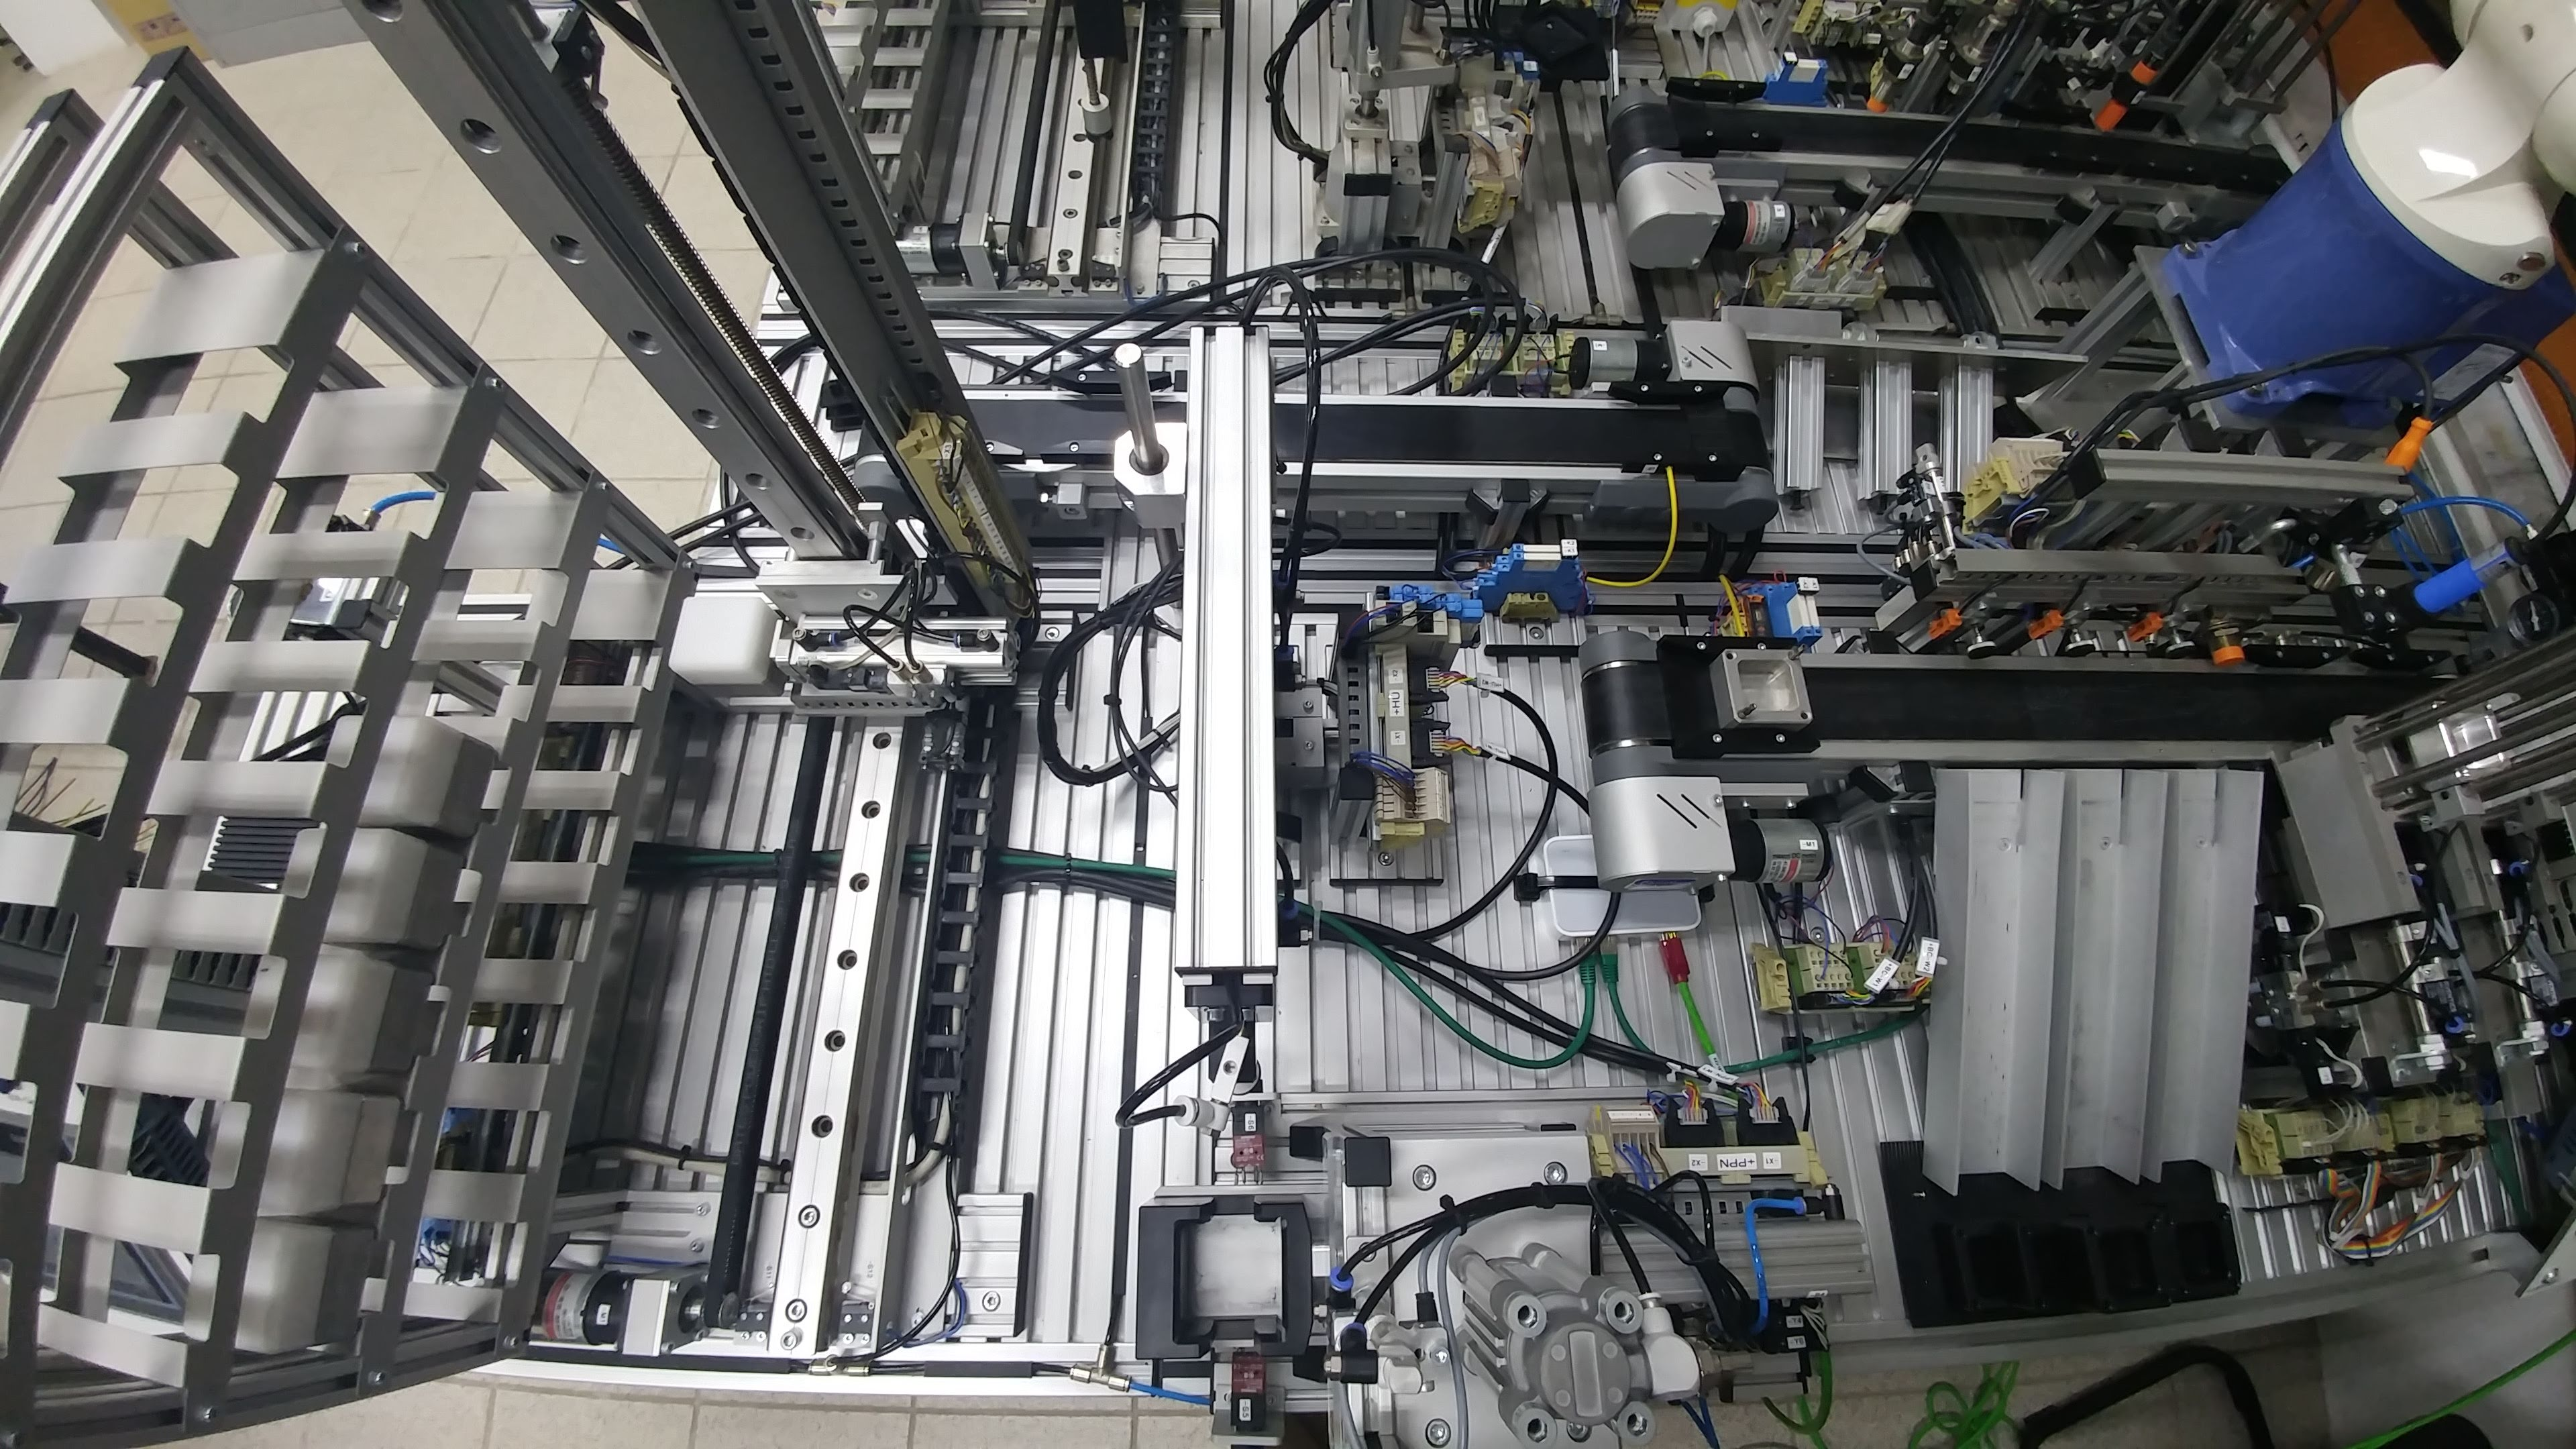
\includegraphics[trim={20cm 0 30cm 20cm},clip,width=0.8\textwidth]{maquete/armAngles.jpg}
    };
    % \draw[red,ultra thick,rounded corners] (0,0) rectangle (9.4,6.2);
    \begin{scope}[x={(image.south east)},y={(image.north west)}]
        % \draw[help lines,xstep=.1,ystep=.1] (0,0) grid (1,1);
        % \foreach \x in {0,1,...,9} { \node [anchor=north] at (\x/10,0) {0.\x}; }
        % \foreach \y in {0,1,...,9} { \node [anchor=east] at (0,\y/10) {0.\y}; }a
        
      
        \draw[red,->,>=stealth,very thick] (0.48,0.9) -- ++(-50:0.7);
        \draw[red,->,>=stealth,very thick] (0.48,0.9) -- ++(-95:0.7);
        \draw[red,->,>=stealth,very thick] (0.48,0.9) -- ++(-120:0.7);

        \draw[fill=red, fill opacity=0.2,draw=none] (0.48,0.9) -- ([shift=(-50:0.5)]0.48,0.9) arc (-50:-95:0.5);
        \draw[fill=blue, fill opacity=0.2,draw=none] (0.48,0.9) -- ([shift=(-95:0.5)]0.48,0.9) arc (-95:-120:0.5);

        \draw [fill,white,fill opacity=0.7,draw=none] (0.02,0.23) rectangle ++ (0.35,0.06);
        \draw [black] (0.2,0.25) node {\tiny \textbf{STORAGE\_ANGLE\_BEFORE}};

        \draw [fill,white,fill opacity=0.7,draw=none] (0.25,0.13) rectangle ++ (0.3,0.06);
        \draw [black] (0.4,0.15) node {\tiny \textbf{PRESS\_ANGLE\_AFTER}};

        \draw [fill,white,fill opacity=0.7,draw=none] (0.7,0.28) rectangle ++ (0.3,0.06);
        \draw [black] (0.85,0.3) node {\tiny \textbf{PRESS\_ANGLE\_BEFORE}};

        \draw [fill,white,fill opacity=0.7,draw=none] (0.1,0.82) rectangle  (0.2,0.96);
        \draw [red,thick] ([shift=(0:0.03)]0.15,0.9) arc (0:180:0.03);
        \draw[black,->,>=stealth,very thick] (0.15,0.85) -- ++(0,0.1);
        \draw [red,->,>=stealth,thick] ([shift=(0:-0.03)]0.15,0.9) arc (-180:-20:0.03);

      \end{scope}
  \end{tikzpicture}
  \caption{Sensors}
\end{figure}

Identification algorithm as seen in \cite{moreira2018enhanced}
\begin{algorithm2e}
  \caption{Identification Algorithm}\label{alg:identification}
\KwIn
{%
Modified observed paths $p_i^k$, for i= 1,\dots,$r$
}
\KwOut
{%
DAOCT = $($\XSet,\SigmaSet,\OmegaSet,\ffunction,\lambdafunction,\RSet,\thetafunction,\xZero,\XfSet$)$
}
\BlankLine
Create an initial state $x_0$, and define $\lambda(x_0) = \tilde{\lambda}(x_0) =
y_{1,1}$

$X = \{ x_0\}, X_f = \emptyset$

\For{$i = 1$ \KwTo $r$}
{
\For{$j = 1$ \KwTo $l_i - 1$}
{
  Find the State $x \in X $ such that $\tilde{\lambda}(x) = y_{i,j+1}$

  \eIf{$\tilde{\lambda}(x) \neq y_{i,j+1}$ for all $ x \in X$}
  { Create state $x^\prime$ and define $\tilde{\lambda}(x^\prime) = y_{i,j+1}$

$X = X \cup \{ x^\prime\}$

$\lambda(x^\prime) = \tilde{\lambda_l}(x^\prime)$

}
{
  Find $x^\prime \in X$ such that $\tilde{\lambda}(x^\prime) = y_{i,j+1}$
}
$f(x,\sigma_{i,j}) = x^\prime$

Add $i$ to $\theta(x,\sigma_{i,j})$

\If{$j = l_i - 1$}
{
  $X_f = X_f \cup \{x^\prime\}$
}
}
}
\end{algorithm2e}

% \begin{table}[H]
%   \centering
%   \caption{table}
%   \begin{tabular}{cc}
%     \label{tab:tab1}
%     \hypertarget{tab:1}{}
%     Transição&Significado\\
%     \hline \\
%     \hyperlink{partialNet:t1}{\hypertarget{partialTable:t1}{$t_{1}$}}&Test\\
%     \hyperlink{partialNet:p1}{\hypertarget{partialTable:p1}{$p_{1}$}}&balbalbal\\
%     \hyperlink{partialNet:p0m2}{\hypertarget{partialTable:p0m2}{$p_{0}$}}&balbalbal
%   \end{tabular}
% \end{table}

% \newpage
% \begin{figure}[h]
%   \centering
%   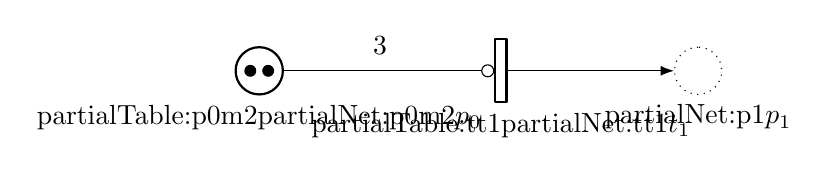
\begin{tikzpicture}[>=latex',line join=bevel,]
%%
\node (p0m2) at (27.0bp,18.0bp) [draw,ellipse,place, tokens=2, label=above:, label=left:\hyperlink{partialTable:p0m2}{\hypertarget{partialNet:p0m2}{$p_{0}$}},rotate=90] {};
  \node (tt1) at (114.0bp,18.0bp) [draw,ellipse,timedtransition, label=above:, label=left:\hyperlink{partialTable:tt1}{\hypertarget{partialNet:tt1}{$t_{1}$}},rotate=90] {};
  \node (ep1) at (185.0bp,18.0bp) [draw,ellipse,extPlace, label=above:, label=left:\hyperlink{partialNet:p1}{$p_{1}$},rotate=90] {};
  \draw [-Latex,inhibitor] (p0m2) ..controls (54.05bp,18.0bp) and (76.966bp,18.0bp)  .. (tt1);
  \definecolor{strokecol}{rgb}{0.0,0.0,0.0};
  \pgfsetstrokecolor{strokecol}
  \draw (70.5bp,27.0bp) node {3};
  \draw [-Latex] (tt1) ..controls (141.25bp,18.0bp) and (147.94bp,18.0bp)  .. (ep1);
%
\end{tikzpicture}

%   \caption{example }
%   \label{fig:example}
% \end{figure}

% \newpage
% \begin{figure}[h]
%   \centering
%   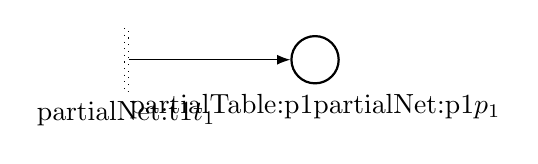
\begin{tikzpicture}[>=latex',line join=bevel,]
%%
\node (et1) at (27.0bp,18.0bp) [draw,ellipse,extTransition, label=above:, label=left:\hyperlink{partialNet:t1}{$t_{1}$},rotate=90] {};
  \node (p1) at (95.0bp,18.0bp) [draw,ellipse,place, label=above:, label=left:\hyperlink{partialTable:p1}{\hypertarget{partialNet:p1}{$p_{1}$}},rotate=90] {};
  \draw [-Latex] (et1) ..controls (54.266bp,18.0bp) and (57.727bp,18.0bp)  .. (p1);
%
\end{tikzpicture}

%   \caption{example }
%   \label{fig:example}
% \end{figure}

% \newpage

% \begin{figure}[H]
%   \centering
%   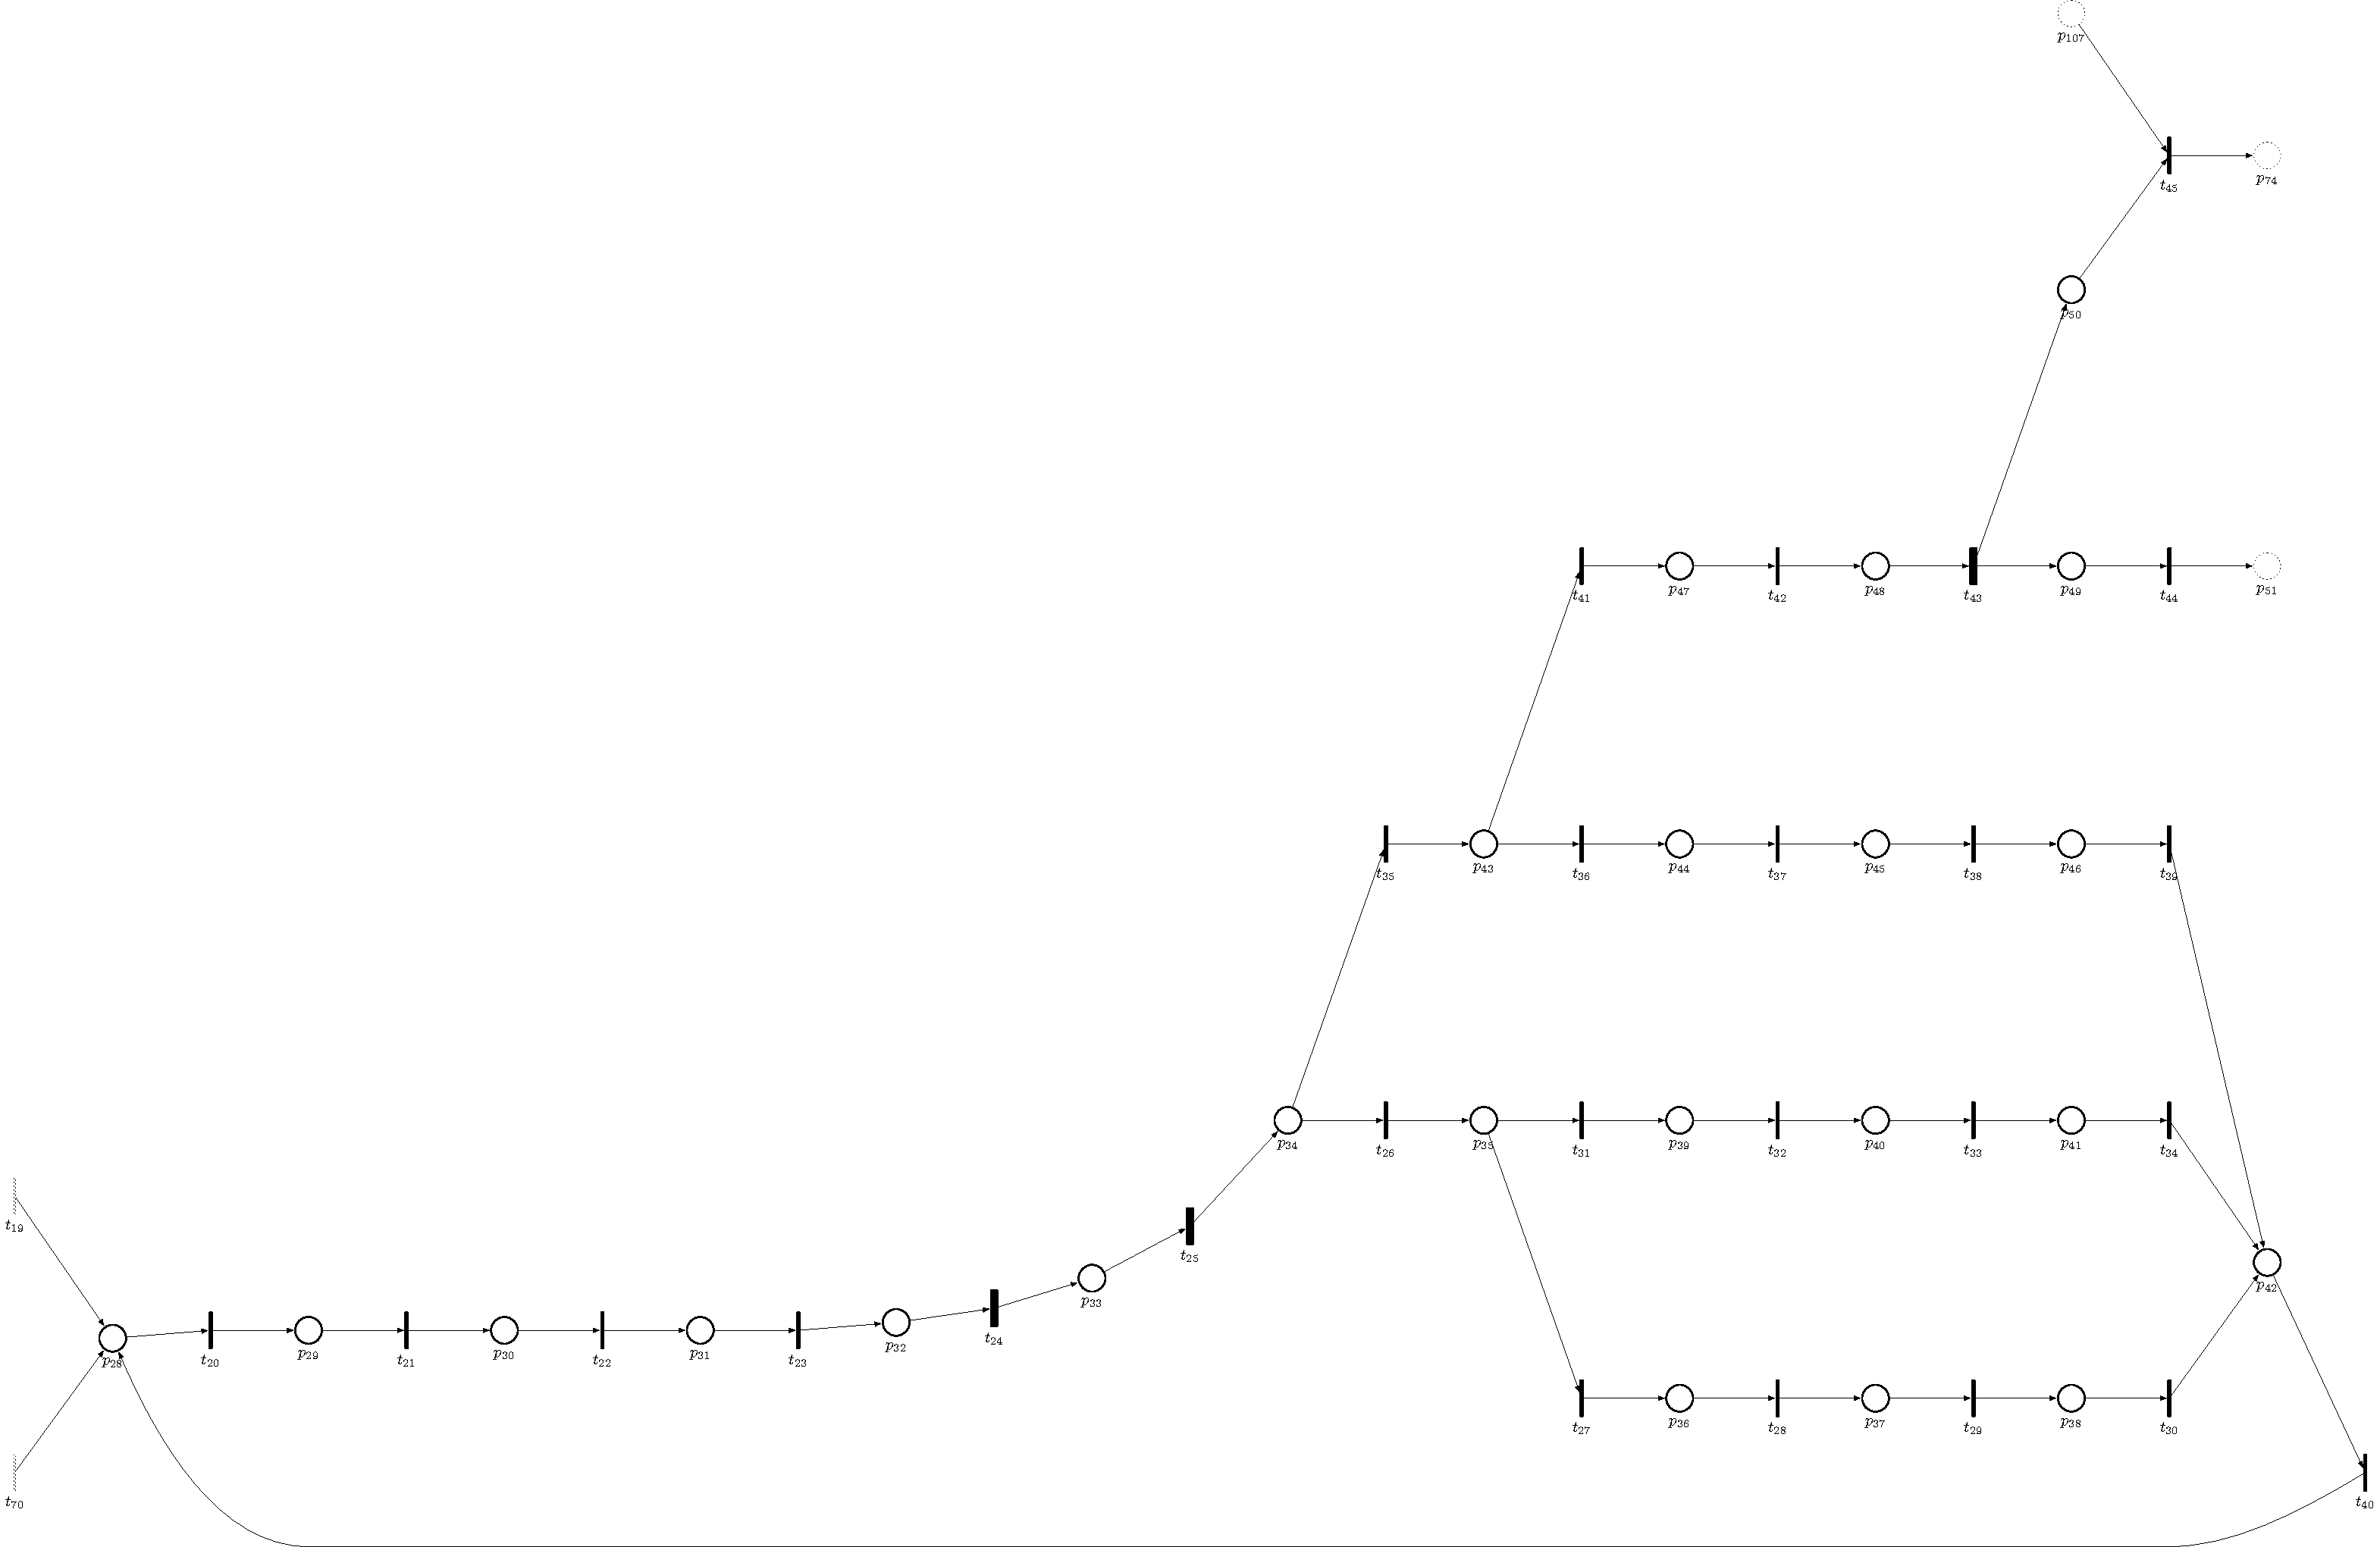
\includegraphics{../../figures/petriNet/dot/2-metalv/metalv.pdf}
%   \caption{qlksdjf}
%   \label{fig:example}
% \end{figure}


% \begin{figure}[H]
%   \centering
%   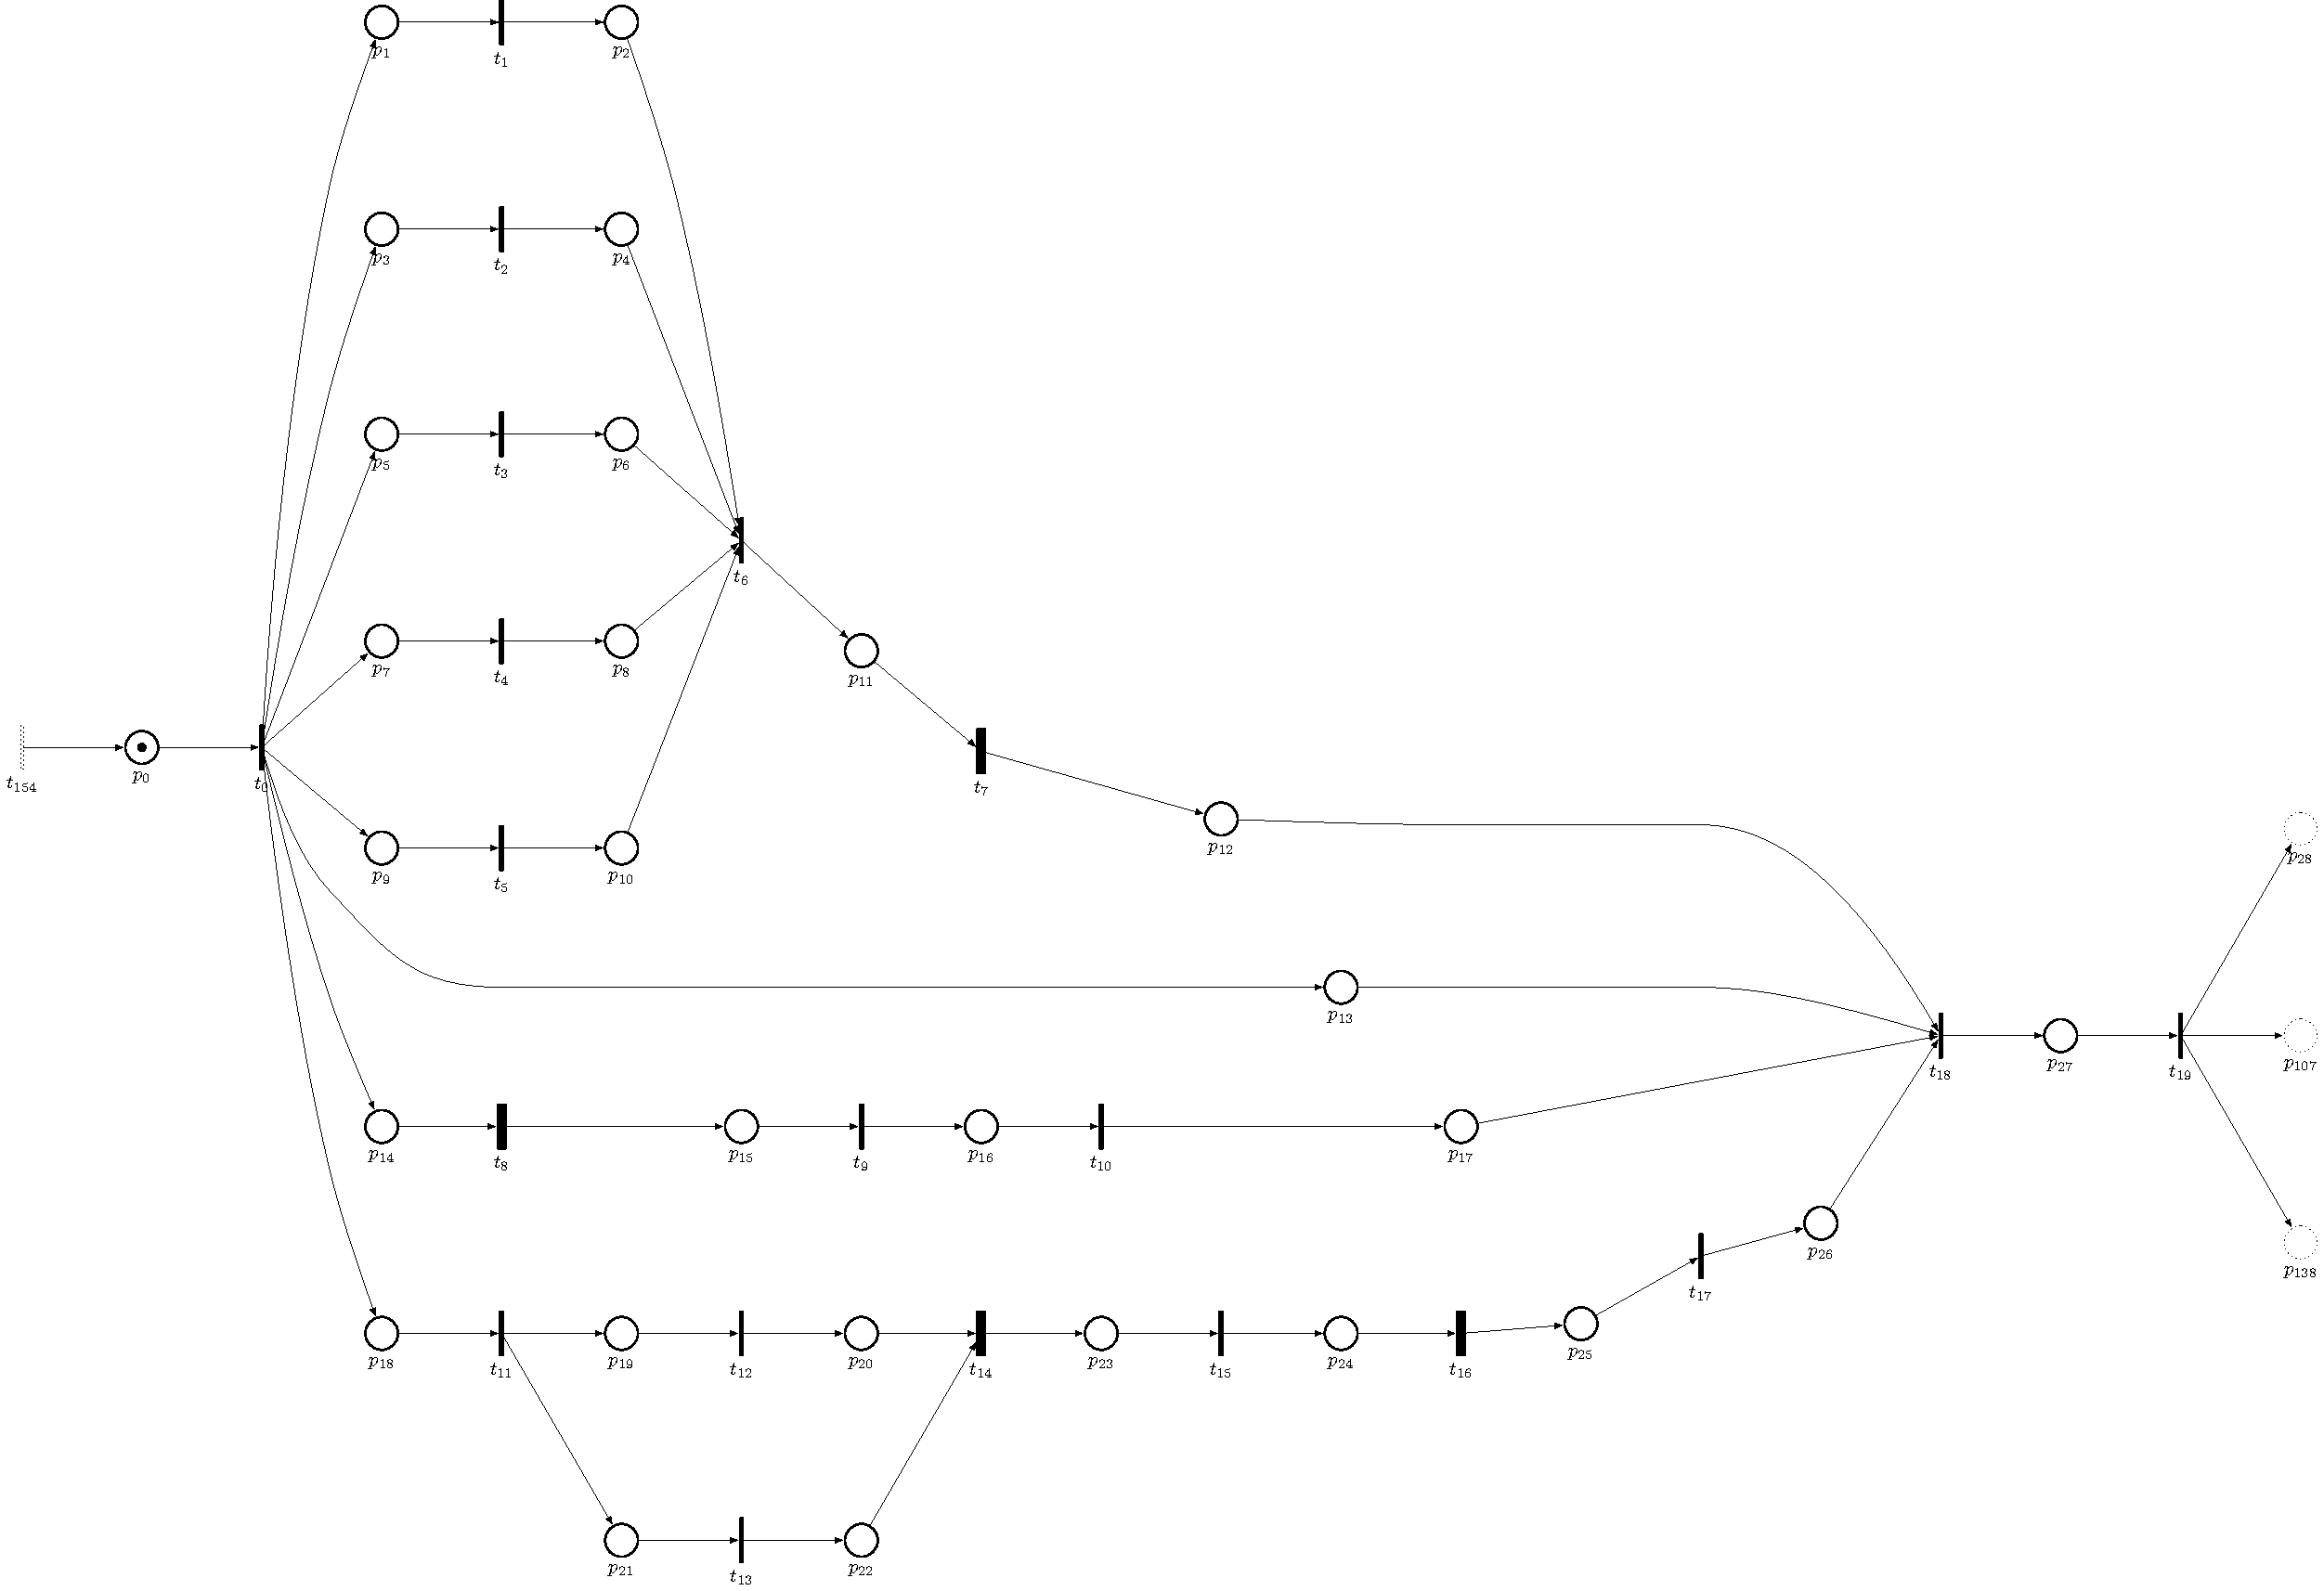
\includegraphics[width=0.4\textwidth]{../../figures/partial/initial.tikz}
%   \caption{petri net bal}
%   \label{fig:petrinetexample}
% \end{figure}

% \addtikzfigure{../../figures/petriNet/partial/initial}
% {Petri net of cube storage module.}
% {petri_initialization}

% \addtikzfigure{../../figures/petriNet//partial/metalv}
% {Petri net of metal cube half sorting module.}
% {petri_initialization}

\begin{table}[htbp]
\caption{Initialization Module Places.}
\centering
\begin{tabular}{M{5cm}M{10cm}}
Places & Meaning\\
\hline
\hyperlink{partialNet:p0m1}{\hypertarget{partialTable:p0m1}{$p_{0}$}} & System Stopped\\
\hyperlink{partialNet:p1}{\hypertarget{partialTable:p1}{$p_{1}$}} & Retract MAG1's Cylinder *\\
\hyperlink{partialNet:p2}{\hypertarget{partialTable:p2}{$p_{2}$}} & MAG1's Cylinder Retracted\\
\hyperlink{partialNet:p3}{\hypertarget{partialTable:p3}{$p_{3}$}} & Retract MAG2's Cylinder *\\
\hyperlink{partialNet:p4}{\hypertarget{partialTable:p4}{$p_{4}$}} & MAG2's Cylinder Retracted\\
\hyperlink{partialNet:p5}{\hypertarget{partialTable:p5}{$p_{5}$}} & Retract Right Discharge Cylinder *\\
\hyperlink{partialNet:p6}{\hypertarget{partialTable:p6}{$p_{6}$}} & Right Discharge Cylinder Retracted\\
\hyperlink{partialNet:p7}{\hypertarget{partialTable:p7}{$p_{7}$}} & Retract Center Discharge Cylinder\\
\hyperlink{partialNet:p8}{\hypertarget{partialTable:p8}{$p_{8}$}} & Center Discharge Cylinder Retracted\\
\hyperlink{partialNet:p9}{\hypertarget{partialTable:p9}{$p_{9}$}} & Retract Left Discharge Cylinder *\\
\hyperlink{partialNet:p10}{\hypertarget{partialTable:p10}{$p_{10}$}} & Left Discharge Cylinder Retracted\\
\hyperlink{partialNet:p11}{\hypertarget{partialTable:p11}{$p_{11}$}} & Turn Conveyor Belt On (Reverse)\\
\hyperlink{partialNet:p12}{\hypertarget{partialTable:p12}{$p_{12}$}} & No Pieces On Conveyor Belt\\
\hyperlink{partialNet:p13}{\hypertarget{partialTable:p13}{$p_{13}$}} & Reset Variables\\
\hyperlink{partialNet:p14}{\hypertarget{partialTable:p14}{$p_{14}$}} & Raise Press\\
\hyperlink{partialNet:p15}{\hypertarget{partialTable:p15}{$p_{15}$}} & Open Safety Door\\
\hyperlink{partialNet:p16}{\hypertarget{partialTable:p16}{$p_{16}$}} & Extend Assembly Unit Holder\\
\hyperlink{partialNet:p17}{\hypertarget{partialTable:p17}{$p_{17}$}} & Assembly Unit Ready\\
\hyperlink{partialNet:p18}{\hypertarget{partialTable:p18}{$p_{18}$}} & Arm Lowered and Retracted, and Storage Unit Retracted\\
\hyperlink{partialNet:p19}{\hypertarget{partialTable:p19}{$p_{19}$}} & Move Storage Unit to the Right\\
\hyperlink{partialNet:p20}{\hypertarget{partialTable:p20}{$p_{20}$}} & Storage Unit ready ( horizontal )\\
\hyperlink{partialNet:p21}{\hypertarget{partialTable:p21}{$p_{21}$}} & Move Storage Device Downwards\\
\hyperlink{partialNet:p22}{\hypertarget{partialTable:p22}{$p_{22}$}} & Storage Unit ready ( vertical )\\
\hyperlink{partialNet:p23}{\hypertarget{partialTable:p23}{$p_{23}$}} & Rotate Arm CCW\\
\hyperlink{partialNet:p24}{\hypertarget{partialTable:p24}{$p_{24}$}} & Turn HSC Off ( Arm Stopped )\\
\hyperlink{partialNet:p25}{\hypertarget{partialTable:p25}{$p_{25}$}} & Rotate Arm CW\\
\hyperlink{partialNet:p26}{\hypertarget{partialTable:p26}{$p_{26}$}} & Arm Stopped facing conveyor belt\\
\hyperlink{partialNet:p27}{\hypertarget{partialTable:p27}{$p_{27}$}} & System Ready\\
\end{tabular}
\end{table}


\begin{table}[H]
\caption{Initialization Module Transitions.}
\centering
\begin{tabular}{M{5cm}M{10cm}}
Transitions & Meaning\\
\hline
\hyperlink{partialNet:t0}{\hypertarget{partialTable:t0}{$t_{0}$}} & Initialization Button\\
\hyperlink{partialNet:t1}{\hypertarget{partialTable:t1}{$t_{1}$}} & MAG1's Cylinder Retracted\\
\hyperlink{partialNet:t2}{\hypertarget{partialTable:t2}{$t_{2}$}} & MAG2's Cylinder Retracted\\
\hyperlink{partialNet:t3}{\hypertarget{partialTable:t3}{$t_{3}$}} & Right Discharge Cylinder Retracted\\
\hyperlink{partialNet:t4}{\hypertarget{partialTable:t4}{$t_{4}$}} & Center Discharge Cylinder Retracted\\
\hyperlink{partialNet:t5}{\hypertarget{partialTable:t5}{$t_{5}$}} & Left Discharge Cylinder Retracted\\
\hyperlink{partialNet:t6}{\hypertarget{partialTable:t6}{$t_{6}$}} & \\
\hyperlink{partialNet:tt7}{\hypertarget{partialTable:tt7}{$t_{7}$}} & T=12s\\
\hyperlink{partialNet:tt8}{\hypertarget{partialTable:tt8}{$t_{8}$}} & T=2.5s\\
\hyperlink{partialNet:t9}{\hypertarget{partialTable:t9}{$t_{9}$}} & Safety Door Opened\\
\hyperlink{partialNet:t10}{\hypertarget{partialTable:t10}{$t_{10}$}} & Assembly Unit Holder Extended\\
\hyperlink{partialNet:t11}{\hypertarget{partialTable:t11}{$t_{11}$}} & Storage Unit Retracted and Arm Lowered and Retracted\\
\hyperlink{partialNet:t12}{\hypertarget{partialTable:t12}{$t_{12}$}} & Storage Unit Right Limit Switch\\
\hyperlink{partialNet:t13}{\hypertarget{partialTable:t13}{$t_{13}$}} & Storage Unit Inferior Limit Switch\\
\hyperlink{partialNet:tt14}{\hypertarget{partialTable:tt14}{$t_{14}$}} & T=2s\\
\hyperlink{partialNet:t15}{\hypertarget{partialTable:t15}{$t_{15}$}} & Inductive Sensor Arm\\
\hyperlink{partialNet:tt16}{\hypertarget{partialTable:tt16}{$t_{16}$}} & T=1s\\
\hyperlink{partialNet:t17}{\hypertarget{partialTable:t17}{$t_{17}$}} & ARMCOUNTER <= BELT\_ANGLE\_CW\\
\hyperlink{partialNet:t18}{\hypertarget{partialTable:t18}{$t_{18}$}} & \\
\hyperlink{partialNet:t19}{\hypertarget{partialTable:t19}{$t_{19}$}} & Start Button\\
\end{tabular}
\end{table}


\begin{longtable}{M{5cm}M{10cm}}
\caption{Metal Half-cube Selection Module Places.} \label{tab:metalvPlaces}
\\
Places & Meaning\\
\hline
\endfirsthead
\multicolumn{2}{l}{Continued from previous page} \\
\hline

Places & Meaning \\

\hline
\endhead
\hline\multicolumn{2}{r}{Continued on next page} \\
\endfoot
\endlastfoot
\hline
\hyperlink{partialNet:p28}{\hypertarget{partialTable:p28}{$p_{28}$}} & MAG1 Empty\\
\hyperlink{partialNet:p29}{\hypertarget{partialTable:p29}{$p_{29}$}} & MAG1 Not Empty\\
\hyperlink{partialNet:p30}{\hypertarget{partialTable:p30}{$p_{30}$}} & Extend MAG1's Cylinder *\\
\hyperlink{partialNet:p31}{\hypertarget{partialTable:p31}{$p_{31}$}} & Retract MAG1's Cylinder *\\
\hyperlink{partialNet:p32}{\hypertarget{partialTable:p32}{$p_{32}$}} & MAG1's Cylinder Retracted\\
\hyperlink{partialNet:p33}{\hypertarget{partialTable:p33}{$p_{33}$}} & Turn Conveyor Belt On\\
\hyperlink{partialNet:p34}{\hypertarget{partialTable:p34}{$p_{34}$}} & \\
\hyperlink{partialNet:p35}{\hypertarget{partialTable:p35}{$p_{35}$}} & Plastic Half-cube\\
\hyperlink{partialNet:p36}{\hypertarget{partialTable:p36}{$p_{36}$}} & Turn Conveyor Belt On\\
\hyperlink{partialNet:p37}{\hypertarget{partialTable:p37}{$p_{37}$}} & Extend Right Discharge Cylinder *\\
\hyperlink{partialNet:p38}{\hypertarget{partialTable:p38}{$p_{38}$}} & Retract Right Discharge Cylinder *\\
\hyperlink{partialNet:p39}{\hypertarget{partialTable:p39}{$p_{39}$}} & Turn Conveyor Belt On\\
\hyperlink{partialNet:p40}{\hypertarget{partialTable:p40}{$p_{40}$}} & Extend Center Discharge Cylinder *\\
\hyperlink{partialNet:p41}{\hypertarget{partialTable:p41}{$p_{41}$}} & Retract Center Discharge Cylinder *\\
\hyperlink{partialNet:p42}{\hypertarget{partialTable:p42}{$p_{42}$}} & \\
\hyperlink{partialNet:p43}{\hypertarget{partialTable:p43}{$p_{43}$}} & Metal Half-cube\\
\hyperlink{partialNet:p44}{\hypertarget{partialTable:p44}{$p_{44}$}} & Turn Conveyor Belt On\\
\hyperlink{partialNet:p45}{\hypertarget{partialTable:p45}{$p_{45}$}} & Extend Left Discharge Cylinder *\\
\hyperlink{partialNet:p46}{\hypertarget{partialTable:p46}{$p_{46}$}} & Retract Left Discharge Cylinder *\\
\hyperlink{partialNet:p47}{\hypertarget{partialTable:p47}{$p_{47}$}} & Turn Conveyor Belt On\\
\hyperlink{partialNet:p48}{\hypertarget{partialTable:p48}{$p_{48}$}} & Turn Conveyor Belt On\\
\hyperlink{partialNet:p49}{\hypertarget{partialTable:p49}{$p_{49}$}} & Metal Half-cube Ready\\
\hyperlink{partialNet:p50}{\hypertarget{partialTable:p50}{$p_{50}$}} & Conveyor Belt Stopped\\
\end{longtable}


\begin{table}[H]
\caption{Metal Half-cube Selection Module Transitions.}
\centering
\begin{tabular}{M{5cm}M{10cm}}
Transitions & Meaning\\
\hline
\hyperlink{partialNet:t20}{\hypertarget{partialTable:t20}{$t_{20}$}} & \(\overline{\mbox{MAG1 Empty}}\)\\
\hyperlink{partialNet:t21}{\hypertarget{partialTable:t21}{$t_{21}$}} & \\
\hyperlink{partialNet:t22}{\hypertarget{partialTable:t22}{$t_{22}$}} & MAG1's Cylinder Extended \(\uparrow\)\\
\hyperlink{partialNet:t23}{\hypertarget{partialTable:t23}{$t_{23}$}} & MAG1's Cylinder Retracted \(\uparrow\)\\
\hyperlink{partialNet:tt24}{\hypertarget{partialTable:tt24}{$t_{24}$}} & T=0.5s\\
\hyperlink{partialNet:tt25}{\hypertarget{partialTable:tt25}{$t_{25}$}} & Presence \(\uparrow\) T=0.5s\\
\hyperlink{partialNet:t26}{\hypertarget{partialTable:t26}{$t_{26}$}} & \(\overline{\mbox{Metallic Sensor}}\)\\
\hyperlink{partialNet:t27}{\hypertarget{partialTable:t27}{$t_{27}$}} & \(\overline{\mbox{White Color Sensor}}\)\\
\hyperlink{partialNet:t28}{\hypertarget{partialTable:t28}{$t_{28}$}} & Proximity Sensor Left Discharge Cylinder \(\uparrow\)\\
\hyperlink{partialNet:t29}{\hypertarget{partialTable:t29}{$t_{29}$}} & Right Discharge Cylinder Extended\\
\hyperlink{partialNet:t30}{\hypertarget{partialTable:t30}{$t_{30}$}} & Right Discharge Cylinder Retracted\\
\hyperlink{partialNet:t31}{\hypertarget{partialTable:t31}{$t_{31}$}} & White Color Sensor\\
\hyperlink{partialNet:t32}{\hypertarget{partialTable:t32}{$t_{32}$}} & Proximity Sensor Center Discharge Cylinder \(\uparrow\)\\
\hyperlink{partialNet:t33}{\hypertarget{partialTable:t33}{$t_{33}$}} & Center Discharge Cylinder Extended\\
\hyperlink{partialNet:t34}{\hypertarget{partialTable:t34}{$t_{34}$}} & Center Discharge Cylinder Retracted\\
\hyperlink{partialNet:t35}{\hypertarget{partialTable:t35}{$t_{35}$}} & Metallic Sensor\\
\hyperlink{partialNet:t36}{\hypertarget{partialTable:t36}{$t_{36}$}} & Concavity Downwards\\
\hyperlink{partialNet:t37}{\hypertarget{partialTable:t37}{$t_{37}$}} & Proximity Sensor Left Discharge Cylinder \(\uparrow\)\\
\hyperlink{partialNet:t38}{\hypertarget{partialTable:t38}{$t_{38}$}} & Left Discharge Cylinder Extended\\
\hyperlink{partialNet:t39}{\hypertarget{partialTable:t39}{$t_{39}$}} & Left Discharge Cylinder Retracted\\
\hyperlink{partialNet:t40}{\hypertarget{partialTable:t40}{$t_{40}$}} & \\
\hyperlink{partialNet:t41}{\hypertarget{partialTable:t41}{$t_{41}$}} & Concavity Upwards\\
\hyperlink{partialNet:t42}{\hypertarget{partialTable:t42}{$t_{42}$}} & Proximity Sensor End Of Conveyor Belt \(\uparrow\)\\
\hyperlink{partialNet:tt43}{\hypertarget{partialTable:tt43}{$t_{43}$}} & T=0.5s\\
\hyperlink{partialNet:t44}{\hypertarget{partialTable:t44}{$t_{44}$}} & Proximity Sensor End Of Conveyor Belt \(\downarrow\)\\
\hyperlink{partialNet:t45}{\hypertarget{partialTable:t45}{$t_{45}$}} & \\
\end{tabular}
\end{table}


%%% Local Variables:
%%% mode: latex
%%% TeX-master: "../monografia"
%%% End:


\chapter{Introduction}
In a world where the majority of the population lives in industrial societies,
and machines take part on the bulk of the production of almost all goods: from
food to cosmetics and drugs, from toothbrushes to automobiles, 
a well-paced throughput it is crucial, and any non expected halt on the
production or change can be disastrous, producing sometimes multimillionaire debts,
provoking a snowball effect, affecting the economy and consequentially the welfare of the society.

A diverse number of causes of the halt or change of the throughput can be
accounted for. Some are as simple as a power outage, or a component malfunction,
but nowadays there are other players. As the industry \textsl{walks}, or even
better \textsl{runs}, towards the so called Fourth Industrial Revolution, the industry
urges the use of \textit{connected sensors}, since the Internet of Things is the
fashion these days, but the concerns about cyber security are now and again neglected.   
So hackers can infiltrate the system, and depending of the infrastructure
halt or change somehow the production throughput.

Cyber security is not the theme of this thesis but its theme is another important concern to a
well-paced throughput, failure detection.

As great part of the manufacture facilities uses conveyor
belts, pneumatic cylinders and digital sensors, it is very common to see \PLCs



\PLC 




\acr{oi}{oi}{oi}
\oi





khe  the most simple as  In order to prevent these effects lots of 
\todo{ objetivo mostrar que o metodo pode funcionar 
com comportamento paraelo mostrar a escabilidade
}
\doing{the objective of this thesis is to show that the \DAOCT model works with
  systems that presents parallel behavior dividing themand can be used to scalability }
\section{Thesis Outline}
\label{sec:thesisOutline}






%%% Local Variables:
%%% mode: latex
%%% TeX-master: "../monografia.tex"
%%% End:

\chapter{Revisão Bibliográfica}


%%% Local Variables:
%%% mode: latex
%%% TeX-master: "../main"
%%% End:

\chapter{Método Proposto}
\chapter{Resultados e Discussões}
\chapter{Conclusões}

\gls{ECA}
Teste de teste
\begin{table}[H]
  \centering
  \begin{tabular}{cc}
    \label{tab:tab1}
    \hypertarget{tab:1}{}
    Transição&Significado\\
    \hline \\
    \hyperlink{net:1}{$t_{1}$}&Test

  \end{tabular}
  \caption{table}
\end{table}

\backmatter
\bibliographystyle{coppe-unsrt}
\nocite{*}
\bibliography{bibliography}

\appendix
\chapter{Algumas Demonstrações}
\end{document}
